% === RobustUAVs.ai Technical Documentation v1 ============================
%  First release of the platform documentation, written to the same template
%  as RobustIDPS.ai Documentation v5 so the two read as a family.
%
%  Every number in this document was read from the running system or from a
%  committed result file at the time of writing, not transcribed from a plan.
%  Where a quantity is modelled rather than measured, it says so. Where a
%  result is pending on external data, it says that too, and names the file
%  that tracks it. This is the same discipline the platform enforces in code:
%  a page that cannot show a measurement says why rather than showing a
%  plausible substitute.
%
%  Author : Roger Nick Anaedevha
%  Affiliation : Institute of Cyber Intelligent Systems, NRNU MEPhI, Moscow
%  Platform : https://robustuavs.ai
%  Artifact : https://github.com/rogerpanel/RobustUAVs.ai
% ===========================================================================

\documentclass[11pt,a4paper]{article}
\usepackage[margin=1in]{geometry}
\usepackage{mathptmx}
\usepackage{amsmath,amssymb}
\usepackage{booktabs}
\usepackage{graphicx}
\usepackage{tikz}
\usetikzlibrary{shapes.geometric,arrows.meta,positioning,calc,fit,backgrounds}
\usepackage{multirow}
\usepackage{xcolor}
\usepackage{fancyhdr}
\usepackage{enumitem}
\usepackage{tabularx}
\usepackage{float}
\usepackage{listings}
\usepackage[hidelinks,breaklinks]{hyperref}

\definecolor{uavblue}{HTML}{1F4E79}
\definecolor{uavdark}{HTML}{0D2F4F}
\definecolor{uavgrey}{HTML}{F5F5F5}
\definecolor{netcol}{HTML}{1F4E79}
\definecolor{autocol}{HTML}{12785A}
\definecolor{bridgecol}{HTML}{B06000}
\definecolor{accent}{HTML}{8C1414}
\definecolor{okgreen}{HTML}{2E7D32}
\hypersetup{colorlinks=true,linkcolor=uavblue,citecolor=uavblue,urlcolor=uavdark}

\pagestyle{fancy}
\fancyhf{}
\fancyhead[L]{\small\textsc{RobustUAVs.ai --- Technical Documentation v1}}
\fancyhead[R]{\small\thepage}
\fancyfoot[C]{\small \texttt{robustuavs.ai} $\cdot$ every number carries a provenance tag}
\renewcommand{\headrulewidth}{0.4pt}
\renewcommand{\footrulewidth}{0.2pt}

\lstset{
  basicstyle=\ttfamily\footnotesize,
  breaklines=true,
  frame=single,
  framerule=0.4pt,
  rulecolor=\color{black!30},
  backgroundcolor=\color{uavgrey},
  xleftmargin=4pt,
  xrightmargin=4pt,
}

\newcommand{\code}[1]{\texttt{#1}}
\newcommand{\MCR}{\mathrm{MCR}}

\newcommand{\provbox}[1]{%
  \par\medskip\noindent
  \begin{tabular}{@{}p{2.5mm}@{\hspace{3mm}}p{0.93\linewidth}@{}}
  \textcolor{bridgecol}{\rule{2.5mm}{\baselineskip}} & \small\itshape #1
  \end{tabular}\par\medskip}

\title{%
  \vspace{-1cm}
  {\LARGE\bfseries RobustUAVs.ai --- v1}\\[6pt]
  {\large A Cross-Layer UAV Security Platform: Six Unified Corpora,\\
   a Composed Network-to-Navigation Certificate, and a\\
   Provenance-Enforcing Evaluation Surface}}
\author{%
  \textbf{Roger Nick Anaedevha}\\
  Institute of Cyber Intelligent Systems, NRNU MEPhI, Moscow, Russia\\[8pt]
  \normalsize Platform: \url{https://robustuavs.ai} \quad$\cdot$\quad
  Artifact: \url{https://github.com/rogerpanel/RobustUAVs.ai}}
\date{August 2026}

\begin{document}
\maketitle
\thispagestyle{fancy}

% ================================================================
\begin{abstract}
\noindent
RobustUAVs.ai is an open research platform for cross-layer UAV security. It
exists to make one question answerable: \emph{if an attacker stays just below a
network detector's alarm threshold, will the mission still complete, and can
that be proved?} Answering it requires objects no public dataset provides, so
the platform supplies them.

The system spans \textbf{25 interconnected pages} in \textbf{8 sidebar groups},
served by a FastAPI control plane exposing \textbf{41 endpoints} across
\textbf{16 modules}, with an Expo / React~Native client of \textbf{27 screens}
that runs from one source on web, iOS and Android. A registry carries
\textbf{13 models} in five categories: four navigation detectors, two published
baselines, one network detector, five certificates, and the composed guarantee
that chains them.

Three properties distinguish it from a dashboard over a results directory.
First, \textbf{nothing is hard-coded}: every number served traces to a file
under \code{results/} or to a live call into the certificate engine, and a
result that has not been produced returns HTTP~503 with the reason rather than
an interpolated value. Second, \textbf{provenance is mandatory and visible}: the
schema's unit of analysis is the cross-layer pairing, every pairing records how
its causal coupling was established, and every page badges itself
\emph{measured} or \emph{illustrative}. Third, the platform \textbf{reports
against itself}: it states that the number of released
\code{measured\_same\_platform} pairings is currently zero, and it says so on
the page a reviewer would use to check.

The corpus unifies six sources totalling \textbf{431,773 events}, of which
\textbf{200,610 (46.5\%)} were captured on real hardware. The certificate engine
implements four complementary methods and reports the fourth as a form awaiting
its numeric constant rather than filling it. A live fleet simulation flies up to
\textbf{12 aircraft} under \textbf{10 attack classes} with emergent mesh
partitioning, and a six-phase GNSS spoofing process runs interactively. This
document describes what is built, what is measured, what is modelled, and what
is still blocked.
\end{abstract}

\tableofcontents
\newpage

% ================================================================
\section{Introduction}

\subsection{The problem the platform is built around}
UAV security is studied from two directions that do not meet. Network intrusion
detection inspects the traffic carried by the swarm mesh, the command-and-control
link and the on-board bus, and raises an alarm when that traffic looks
malicious. Certified robustness proves that a navigation model's output cannot
move by more than a fixed amount when its sensor input is perturbed by no more
than a given magnitude. The first stops at the alarm and says nothing about the
flight that follows an intrusion it fails to catch. The second takes the
perturbation as given and asks neither where it originates nor how often an
adversary can produce one.

The gap between them is not academic. A detector must tolerate natural jitter to
be usable, so an adversary who stays just under that tolerance is invisible by
construction. What happens to the aircraft afterwards is precisely the question
an operator, an insurer and a regulator need answered, and it is the question
that falls between the two literatures.

\subsection{What the platform contributes}
RobustUAVs.ai is the instrument for closing that gap. It contributes four
things, and the sections that follow describe each in turn.

\begin{enumerate}[leftmargin=1.6em]
\item A \textbf{two-layer schema} whose unit of analysis is the
\emph{cross-layer pairing}: an interval during which a network attack is active,
joined to the interval of degraded navigation it induces, carrying a mandatory
flag recording how strongly that causal link is evidenced
(\S\ref{sec:schema}).
\item A \textbf{corpus} of six public sources unified under that schema by one
lossless adapter each, with a detector-operating-curve harness that makes the
detector's alarm threshold a swept parameter (\S\ref{sec:corpus}).
\item A \textbf{certificate engine} implementing four complementary methods and
the composition that chains a detector threshold to a mission-completion floor
(\S\ref{sec:certificates}).
\item A \textbf{web platform} that serves all of the above, adds live
simulation, and enforces the provenance discipline in the user interface rather
than only in the data (\S\ref{sec:platform} onwards).
\end{enumerate}

\subsection{The one design rule}
Every other decision in this system follows from a single rule:

\provbox{A number is shown with its provenance, or it is not shown. When a
result has not been produced, the platform says which input is missing and where
that gap is tracked. It never substitutes a plausible value.}

This is why a page can return HTTP~503, why the Calibration page deliberately
displays nothing, why every screen carries a \emph{measured} or
\emph{illustrative} badge, and why the corpus page reports a count of zero
against the strongest evidence class. A reviewer who cannot tell a measurement
from a model cannot check the work, and a platform that blurs the two is worse
than no platform.

% ================================================================
\section{System Architecture}
\label{sec:platform}

\subsection{Two-plane architecture}
The system separates a \textbf{research plane} that produces numbers from a
\textbf{control plane} that serves them. The separation is strict and
one-directional: the control plane reads committed artefacts and never computes
a research result on the request path, except for the certificate engine, which
is called live because it is deterministic and fast.

\begin{figure}[H]
\centering
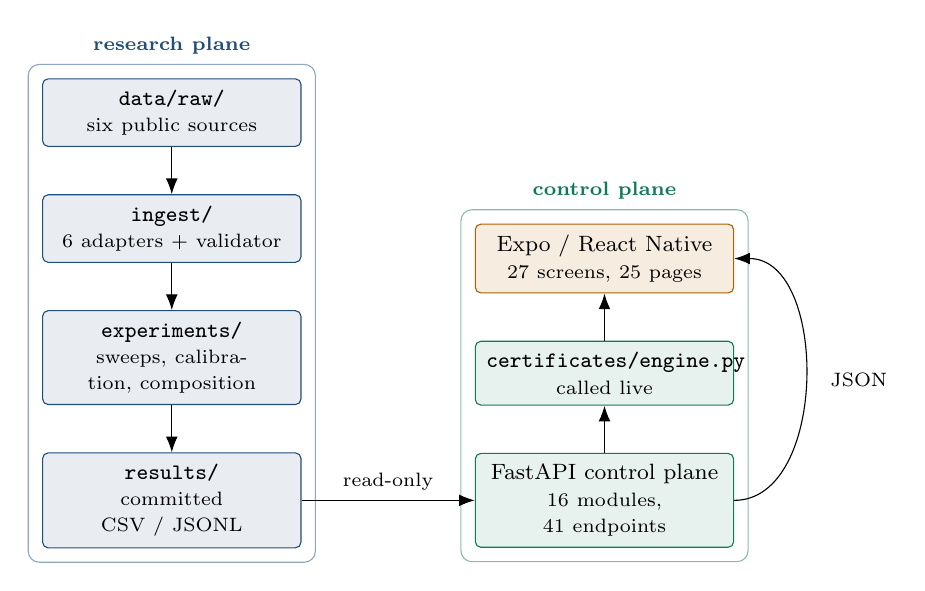
\begin{tikzpicture}[font=\footnotesize,>={Latex[length=2mm]},node distance=6mm,
  box/.style={rounded corners=2pt,draw,align=center,minimum height=8mm,inner sep=4pt,text width=30mm},
  res/.style={box,fill=netcol!10,draw=netcol},
  ctl/.style={box,fill=autocol!10,draw=autocol},
  cli/.style={box,fill=bridgecol!12,draw=bridgecol}]
\node[res] (raw) {\code{data/raw/}\\\scriptsize six public sources};
\node[res,below=of raw] (ing) {\code{ingest/}\\\scriptsize 6 adapters + validator};
\node[res,below=of ing] (exp) {\code{experiments/}\\\scriptsize sweeps, calibration, composition};
\node[res,below=of exp] (out) {\code{results/}\\\scriptsize committed CSV / JSONL};
\node[ctl,right=22mm of out] (api) {FastAPI control plane\\\scriptsize 16 modules, 41 endpoints};
\node[ctl,above=of api] (cert) {\code{certificates/engine.py}\\\scriptsize called live};
\node[cli,above=of cert] (app) {Expo / React Native\\\scriptsize 27 screens, 25 pages};
\draw[->] (raw) -- (ing); \draw[->] (ing) -- (exp); \draw[->] (exp) -- (out);
\draw[->] (out) -- node[above,font=\scriptsize]{read-only} (api);
\draw[->] (api) -- (cert); \draw[->] (cert) -- (app);
\draw[->] (api.east) to[out=0,in=0] node[right,font=\scriptsize,xshift=2mm]{JSON} (app.east);
\begin{scope}[on background layer]
\node[fit=(raw)(out),draw=netcol!50,rounded corners,inner sep=5pt,
  label={[font=\scriptsize\bfseries,text=netcol]above:research plane}]{};
\node[fit=(api)(app),draw=autocol!50,rounded corners,inner sep=5pt,
  label={[font=\scriptsize\bfseries,text=autocol]above:control plane}]{};
\end{scope}
\end{tikzpicture}
\caption{The two planes. Research artefacts flow one way. The control plane
holds no research state of its own, which is what makes every served number
traceable to a committed file.}
\end{figure}

\subsection{Sidebar layout: 8 groups, 25 pages}
\begin{table}[H]
\centering\small
\begin{tabularx}{\linewidth}{@{}p{3.4cm}p{0.8cm}X@{}}
\toprule
\textbf{Group} & \textbf{Pages} & \textbf{Contents} \\
\midrule
Results & 2 & Milestones, Composition \\
UAV / Aerial Defense & 8 & UAV Monitor, Swarm Graph, Fleet Demo, GNSS Spoof Monitor, Certification, Mission Plan, Perception, Dossier \\
Evaluation & 5 & Robustness, Ablations, ROC, Statistics, Calibration \\
Analyse & 1 & Upload \& Analyse \\
Build & 4 & Agent Studio, Interface stability, Mission-distribution sensitivity, Federated Learning \\
Experiments & 2 & Runs, SOC Copilot \\
Corpus & 2 & Overview, Model registry \\
Present & 1 & Cover \\
\midrule
\textbf{Total} & \textbf{25} & across 8 groups \\
\bottomrule
\end{tabularx}
\caption{Navigation structure, read from \code{platform/mobile/src/layout/nav.js}.}
\end{table}

Every page carries a hideable step-by-step help panel written for a reader who
has not seen the page before, telling them what to look at first and what the
page is evidence for. Several also carry a \emph{tip} naming the reviewer
question the page is designed to answer.

\subsection{The 41 endpoints}
\begin{table}[H]
\centering\footnotesize
\begin{tabularx}{\linewidth}{@{}p{3.0cm}X@{}}
\toprule
\textbf{Family} & \textbf{Endpoints} \\
\midrule
Health and registry & \code{/api/health}, \code{/api/models}, \code{/api/models/\{id\}} \\
Results & \code{/api/results}, \code{/api/results/\{name\}} \\
Certificates & \code{/api/certify/staleness} \\
Evaluation & \code{/api/eval/}\{\code{robustness}, \code{ablations}, \code{roc}, \code{statistics}, \code{calibration}, \code{federated}, \code{interface}, \code{mission-distribution}\} \\
UAV surface & \code{/api/uav/}\{\code{overview}, \code{certificates}, \code{dossier}, \code{fleet}, \code{fleet/catalog}, \code{fleet/reset}, \code{fleet/step}, \code{gnss/run}, \code{gnss/run/reset}, \code{gnss/run/step}, \code{gnss/sky}, \code{swarm/snapshots}, \code{mission-plan/review}, \code{perception/catalog}, \code{ew-bench/curves}, \code{ew-bench/operating-point}\} \\
Runs & \code{/api/runners}, \code{/api/runs} (GET, POST), \code{/api/runs/\{id\}}, \code{/api/runs/\{id\}/cancel} \\
Copilot & \code{/api/copilot/}\{\code{tools}, \code{tool/\{name\}}, \code{ask}\} \\
Upload & \code{/api/upload/}\{\code{analyse}, \code{compare}, \code{fly}\} \\
\bottomrule
\end{tabularx}
\caption{The control-plane surface. Interactive documentation is served at
\code{/docs}.}
\end{table}

\subsection{Two response conventions that carry meaning}
\textbf{503 is not an error.} A result endpoint returns \code{503} when the
endpoint exists but its result file has not been produced in this deployment.
The client renders this as ``Not produced in this deployment'' and points at
\code{PENDING\_ON\_DATA.md}. Reporting it as a failure would misrepresent a
data gap as a bug, and those are different things to a reviewer.

\textbf{404 is a version mismatch.} A \code{404} means the client is asking for
something this API does not have, which in practice means the bundle is newer
than the backend. The client says ``Client and API are out of step'' and gives
the redeploy command. Conflating the two sends a reader to the wrong document.

% ================================================================
\section{The Two-Layer Schema}
\label{sec:schema}

The schema exists to solve one problem: six datasets describe different things,
at different rates, with no common clock, and any representation that forced
them into one flat table would have to discard whatever did not fit. It uses
three record kinds, arranged in a hierarchy of increasing interpretation.

\begin{enumerate}[leftmargin=1.6em]
\item An \textbf{Event} is a single observation as its source recorded it,
translated into common field names but never summarised. This layer is
deliberately dumb: it asserts nothing beyond what the source file said. A
\code{native} block preserves every unmapped source column, which is what makes
ingestion provably lossless rather than merely convenient.
\item An \textbf{AttackWindow} is an interval during which one named attack was
active on one layer. This layer asserts that something adversarial was
happening, and when.
\item A \textbf{CrossLayerPairing} joins one network window to one autonomy
window and asserts that the first \emph{caused} the second. This is the only
place in the schema where a causal claim is made, and therefore the only place
carrying a mandatory evidence flag.
\end{enumerate}

\subsection{The \code{pairing\_basis} flag}
\begin{table}[H]
\centering\small
\begin{tabularx}{\linewidth}{@{}p{4.2cm}X@{}}
\toprule
\textbf{Value} & \textbf{Meaning} \\
\midrule
\code{measured\_same\_platform} & Both windows recorded on one testbed. The strongest evidence. \\
\code{physics\_model} & Coupled through a named, versioned physical relation a reviewer can inspect and challenge. \\
\code{synthetic\_alignment} & Aligned by construction, under a stated affine clock map with a bounded error budget. \\
\bottomrule
\end{tabularx}
\end{table}

A reviewer can filter the benchmark by evidence strength rather than trusting an
unaudited join, and a claim can never silently upgrade its own provenance.

\subsection{Three design choices}
Time is always \emph{relative} to each source's capture start, because the
sources share no global clock, and cross-layer alignment happens at the window
level, so a mismatch between a 50\,Hz telemetry stream and a per-flow network
record never forces a lossy resample. Attack labels are \emph{unified} into a
common taxonomy while the verbatim source label is retained in
\code{label\_native}. And every unmapped column is preserved.

Alignment therefore needs a stated rule and a stated error budget, since this is
the step at which a benchmark could silently manufacture, or destroy, the effect
it reports. Attack onsets are anchored under an affine map between the two
relative clocks, with residual misalignment bounded by
$e_{\mathrm{align}}\le0.53$\,s for every released pairing. Crucially, the
quantity the certificate consumes is computed entirely within the network
source, so misalignment can attach a pairing to the wrong autonomy window but
cannot inflate or deflate the certified quantity itself.

% ================================================================
\section{The Corpus and Its Adapters}
\label{sec:corpus}

\begin{table}[H]
\centering\footnotesize
\begin{tabularx}{\linewidth}{@{}p{3.3cm}p{2.4cm}p{1.6cm}rX@{}}
\toprule
\textbf{Source} & \textbf{Acquisition} & \textbf{Layer} & \textbf{Events} & \textbf{Role} \\
\midrule
HCRL UAVCAN & real testbed & network, bus & 200,000 & Bus flooding, fuzzing, replay \\
UAVIDS-2025 & simulation (NS-3) & network, mesh & 122,171 & Large-scale mesh flows \\
UAV-EW-Bench-2026 & simulation (physics) & autonomy & 93,600 & The navigation anchor \\
DATAMUt replay & simulation (event) & network, mesh & 15,392 & The sweepable detector \\
UAV Attack Dataset & \textbf{real testbed} & \textbf{both} & 610 & The only source observing both layers on one airframe \\
UAV-CAS & simulation (twin) & network, mesh & 0 & Adapter ready; release file not reachable \\
\midrule
\textbf{Total} & & & \textbf{431,773} & \textbf{200,610 real (46.5\%)} \\
\bottomrule
\end{tabularx}
\caption{Corpus composition, regenerated by
\code{experiments/provenance\_ledger.py} so the document cannot drift from the
artifact.}
\end{table}

\subsection{The number the platform reports against itself}
Acquisition provenance is the weaker question. The stronger one is how many
\emph{pairings} rest on measurement, and there the honest answer is worse:

\provbox{The number of released \code{measured\_same\_platform} pairings is
currently \textbf{zero}. The UAV Attack Dataset release does not carry
machine-readable attack on/off timestamps, so the adapter cannot emit
\code{AttackWindow} boundaries for it and refuses to infer them. Its three
flights still supply the delay-to-position rate the certificate consumes,
self-referenced to each flight's own pre-attack median, so the headline result
does not depend on closing this gap. But a reader who filters the artifact to
the strongest evidence class will correctly retrieve nothing, and the platform
says so on the Corpus page.}

\subsection{Adapters and the validator}
One adapter per source lives in \code{ingest/}, and
\code{ingest/validate.py} is the gate: nothing enters \code{results/}
unvalidated. \code{experiments/run\_real\_corpus.sh} runs the whole pipeline
and is idempotent; a stage whose inputs are absent is skipped with a message
rather than substituted.

\provbox{A caution that cost us a result. The third-party detector demo
\emph{appends} to its summary CSV. An early sweep harness therefore averaged
every previous operating point into the current one, and the symptom was recall
\emph{increasing} with the threshold, which a threshold detector cannot exhibit.
\code{experiments/sweep\_full.py} now uses a fresh working directory per point.
Anyone reimplementing the sweep should do the same.}

% ================================================================
\section{Models and Certificates}
\label{sec:certificates}

\subsection{The registry: 13 models in five categories}
\begin{table}[H]
\centering\small
\begin{tabularx}{\linewidth}{@{}p{2.6cm}p{1.3cm}X@{}}
\toprule
\textbf{Category} & \textbf{Count} & \textbf{Members} \\
\midrule
navigation & 4 & \code{m1\_ct\_tgnn}, \code{m4\_mambashield}, \code{m6\_uc\_hgp}, \code{m7\_fedgtd} \\
baseline & 2 & \code{caf\_cnn}, \code{seq2seq\_tr} \\
network & 1 & \code{datamut} \\
certificate & 5 & \code{cert\_gronwall}, \code{cert\_smoothing}, \code{cert\_staleness}, \code{cert\_mwu}, \code{cert\_pacbayes} \\
composition & 1 & \code{composed} \\
\bottomrule
\end{tabularx}
\end{table}

Each card carries a \code{provenance} and a \code{certificate\_status} field, a
\code{constants} block, and a \code{caveat}. The caveat is not decoration: it is
where a model states what it cannot do.

\subsection{The composition}
The chain the platform serves is
\[
\theta \;\longmapsto\; \Delta(\theta) \;\longmapsto\; \delta(\theta)
\;\longmapsto\; \MCR \ge f\big(\delta(\theta)\big),
\]
read left to right: a detector's alarm threshold $\theta$ bounds the residual
undetected attack $\Delta(\theta)$; the residual maps to a bounded perturbation
$\delta(\theta)$ on the navigation input; and a Lipschitz--Grönwall
trajectory-tube argument turns that bounded input into a guaranteed
Mission-Completion-Rate floor.

\provbox{The chain is not a theorem end to end. Its first and last links are
proved; the middle link, $\Delta\mapsto\delta$, is an \emph{empirical
calibration}. The platform and the accompanying manuscript both describe the
result as a conditional guarantee under an empirically calibrated interface,
and not as end-to-end certified security.}

\subsection{Four certificates, and why one is not enough}
\begin{table}[H]
\centering\footnotesize
\begin{tabularx}{\linewidth}{@{}p{2.9cm}p{2.6cm}X@{}}
\toprule
\textbf{Certificate} & \textbf{Bounds} & \textbf{Regime it covers} \\
\midrule
Lipschitz--Grönwall & the trajectory & Deterministic, bounded disturbance. The only one giving a per-instant geometric envelope, so the only one that discharges the corridor test. \\
Randomized smoothing & a decision at a point & Where the budget is known only statistically. \\
PAC-Bayes & the model & The gap between the training mission mix and this sortie. \\
MWU regret & the time axis & Cumulative loss against an \emph{adapting} jammer. Vacuous at any single instant. \\
\bottomrule
\end{tabularx}
\end{table}

Because a trajectory, a decision, a model and a policy sequence are distinct
objects, the four compose by conjunction rather than selection: a deployment
reads its floor as the pointwise minimum, and the binding term identifies which
assumption is closest to failing.

\subsection{Instantiated constants}
\begin{table}[H]
\centering\small
\begin{tabularx}{\linewidth}{@{}p{4.6cm}p{2.6cm}X@{}}
\toprule
\textbf{Constant} & \textbf{Value} & \textbf{Provenance} \\
\midrule
Lipschitz, measured local & $L = 1.181$ & measured on visited trajectories \\
Lipschitz, global power iteration & $\hat L = 0.983$ & \emph{not used}: smaller, so it would flatter every bound \\
Grönwall radius at $T_c = 1$\,s & $0.1535$ & derived \\
Randomized-smoothing radius & $0.44$ at $\sigma = 0.25$ & measured on the trained checkpoint \\
MWU policy set & $|S| = 4$ & stated \\
PAC-Bayes KL & \textbf{pending} & flagged, not substituted \\
Interface rate $\gamma$ (supremum) & $1.625$\,m/s & 674 post-onset samples, real flights \\
Residual budget saturation & $\le 4.84$\,s & 15,392 observed hops \\
\bottomrule
\end{tabularx}
\end{table}

The Lipschitz row is worth dwelling on. The local constant is the \emph{larger}
of the two, so it widens the trajectory tube and narrows the certified window.
Quoting the global one would flatter every bound reported, which is why the
platform uses the local value and says why.

% ================================================================
\section{The Interface Characterisation Campaign}

The composition consumes $\gamma$, the metres of position error accrued per
second of degraded navigation input, and the platform's most consequential
empirical question is whether $\gamma$ is a single number. It is not.

\subsection{The estimator decides the answer}
Two estimators are available and they disagree qualitatively. Writing $e(t)$ for
position error and $t_0$ for attack onset,
\[
\gamma_{\mathrm{cum}}(t)=\frac{e(t)}{t-t_0},
\qquad
\gamma_{\Delta}(t)=\frac{e(t)-e(t_0)}{t-t_0}.
\]
Onset is declared when the error crosses a detection threshold, so $e(t_0)$ is
not zero: it is $0.64$\,m for jamming at the receiver and $9.27$\,m for
spoofing. Dividing that pre-existing offset by a small $t-t_0$ makes
$\gamma_{\mathrm{cum}}$ diverge, reaching $8.6$\,m/s below one second.

\provbox{That number is an artifact of the detector, not a property of the
attack, and reporting it would have been a serious error: $8.6$\,m/s exceeds
$\gamma_{\mathrm{req}} = 6.14$\,m/s and would have declared the framework
unusable on the strength of a measurement artifact. The delay budget is
responsible only for error the attacker \emph{causes}, so
$\gamma_{\Delta}$ is the estimator the certificate is entitled to. Both are kept
in the per-sample output so the contrast can be audited.}

\subsection{What $\gamma$ depends on}
Over 674 post-onset samples, $\gamma_{\Delta}$ spans $6.1\times$ from median to
supremum and varies systematically:

\begin{table}[H]
\centering\small
\begin{tabularx}{\linewidth}{@{}p{3.4cm}p{3.4cm}X@{}}
\toprule
\textbf{Factor} & \textbf{Effect} & \textbf{Mechanism} \\
\midrule
Attack type & $2.6\times$, spoofing $>$ jamming & Jamming removes information and the estimator dead-reckons; spoofing injects information the estimator accepts, so error accrues at the adversary's chosen rate. \\
Satellite visibility & rises as satellites fall $14\to4$ & Degraded geometry, weaker correction. \\
Staleness & peaks at $\tau\in[5,10)$\,s & Error saturates while the denominator keeps growing. \\
Error signal & only $1.14\times$ & The filter attenuates injected error far less than one might hope. \\
\bottomrule
\end{tabularx}
\end{table}

A descriptive least-squares fit on standardised covariates explains
$R^2 = 0.79$, with physically sensible signs for satellite count ($-0.22$),
staleness ($-0.26$) and airspeed ($+0.12$). No $p$-values are reported: samples
within a flight are strongly autocorrelated and there are two attack flights, so
any nominal significance would be an artifact of the dependence structure.

\subsection{Coverage, stated as a limit}
\begin{table}[H]
\centering\small
\begin{tabularx}{\linewidth}{@{}p{3.2cm}p{2.4cm}X@{}}
\toprule
\textbf{Factor} & \textbf{Status} & \textbf{Detail} \\
\midrule
Attack type & \textcolor{okgreen}{varied} & jamming and spoofing \\
GNSS condition & \textcolor{okgreen}{varied, wide} & satellites $14\to4$, HDOP $0.71\to4.16$, fix $3\to0$ \\
Staleness & \textcolor{okgreen}{varied} & $0.4$ to $\sim70$\,s \\
Airspeed & \textcolor{bridgecol}{poor} & hover; p90 of $\lVert v_{xy}\rVert < 0.65$\,m/s \\
Platform & \textcolor{accent}{\textbf{not varied}} & one PX4 / Pixhawk 4 / Holybro S500 \\
Flight mode & \textcolor{accent}{\textbf{not varied}} & hover / loiter only \\
\bottomrule
\end{tabularx}
\end{table}

A factor the release could not vary is reported as unvaried, never as showing no
effect. The $6.1\times$ spread is therefore a \emph{lower bound} on the
variability a deployment would meet, and the two red rows need flights rather
than analysis.

\subsection{Mission-distribution sensitivity}
MCR is a probability over a distribution of missions, so a bound on it describes
a population and not an individual flight. The platform measures what that
costs. Across nine mission distributions (three profiles $\times$ three receiver
models) at a fixed defence:

\begin{itemize}
\item Marginalised over the whole $0$--$40$\,dB jamming sweep, the spread is
\textbf{0.011}, which looks negligible.
\item Conditional on attack strength, the mission profile alone moves MCR by
\textbf{0.214}, and the receiver model by \textbf{0.154}.
\item The jamming power at which a distribution first falls below the $0.90$
reference ranges from $18.1$ to $27.1$\,dB, a spread of \textbf{9\,dB}, or
roughly a factor of eight in adversary transmit power.
\end{itemize}

Averaging over the adversary hides a dependence that an operator, who flies one
profile against one adversary, lives at.

% ================================================================
\section{The UAV / Aerial Defense Surface}

\subsection{Live fleet simulation}
Up to \textbf{12 aircraft} fly a mission of nominal duration $T = 70$\,s against
a deadline of $(1+\kappa)T$ with $\kappa = 0.25$. The dashboard shows exactly
the number selected, and the fleet is instantiated by sampling from the five
reachable corpus sources rather than from a random generator.

\begin{table}[H]
\centering\footnotesize
\begin{tabularx}{\linewidth}{@{}p{2.4cm}p{1.9cm}X@{}}
\toprule
\textbf{Class} & \textbf{Family} & \textbf{Effect} \\
\midrule
\code{none} & --- & Nominal flight \\
\code{fgsm} & gradient & Single-step gradient sign; cheapest and weakest \\
\code{pgd} & gradient & Iterated with projection; the strong baseline \\
\code{cw} & optimisation & Carlini--Wagner \\
\code{deepfool} & geometric & Minimal-perturbation boundary search \\
\code{gaussian} & noise & Non-adversarial control \\
\code{gnss\_spoof} & RF & Injects a false but consistent fix \\
\code{jam\_link} & RF & Degrades mesh link quality \\
\code{delay\_relay} & network & The class the theorem covers \\
\code{label\_flip} & poisoning & Training-time \\
\bottomrule
\end{tabularx}
\caption{Ten attack classes, from \code{platform/backend/app/uav.py}.}
\end{table}

Mesh degradation is emergent rather than scripted: link residual is the sum of a
measured baseline and accumulated staleness, and a link becomes
\code{delayed} above $0.25$\,s of residual, and \code{jammed} above $5.0$\,s or
when the worse endpoint drops below $25\,\%$ link quality. Jamming two of eight aircraft for 30\,s partitions a nine-link
mesh into four clusters with two isolated, which nothing in the code
instructs it to do.

\provbox{\textbf{Modelled versus measured.} The link residuals are sampled from
real corpus data; the damage rates, return-to-launch thresholds and battery
model are \emph{modelled}. \code{docs/simulation\_architecture.md} lists the
four steps that would move the modelled quantities to measured, the shortest
being per-step detector inference over the already-real link residuals. Every
page badges itself accordingly.}

\subsection{GNSS spoof monitor}
A six-phase interactive process rather than a static diagram: the user steps a
spoofing attack through its phases, watches the satellite geometry and the
estimator response, and can attach a \emph{remark} at any step. The composed
certificate is evaluated live at each phase.

\subsection{The rest of the group}
\textbf{Swarm Graph} renders mesh snapshots with a composite view at $t_4$
showing all selected aircraft together. \textbf{Certification} reads the locked
certificate constants. \textbf{Mission Plan} reviews a proposed corridor and
schedule against the certified window. \textbf{Perception} and \textbf{Dossier}
present the model catalogue and the per-aircraft record.

% ================================================================
\section{Evaluation, Analysis and Copilot}

\subsection{Evaluation group}
\textbf{Robustness} plots the certified floor against the detector threshold,
one series per interface mapping, now including the campaign supremum at
$\gamma = 1.625$\,m/s. \textbf{Ablations} reports how tight $\gamma$ must be for
a given corridor to certify. \textbf{ROC} gives recall and false-positive rate
against the threshold, and the generalisation to any scored detector.
\textbf{Statistics} carries Wilcoxon signed-rank tests with Holm correction.

\textbf{Calibration deliberately shows nothing.} Expected Calibration Error
needs per-hop detector \emph{scores}, and the detector emits a boolean, so no
reliability diagram is derivable from anything committed. The page returns
\code{available: false} with the method, the exact missing input and what would
unblock it. A reviewer asking ``is your detector calibrated?'' gets a straight
answer about why the question cannot yet be answered, which is worth more than a
curve fitted to a boolean.

\subsection{Upload \& Analyse}
A reviewer can upload their own data, up to \textbf{1\,GB} per file across
\textbf{four} slots, and run the platform's models over it. Parsing is streaming with
a reservoir sample of 4,000 rows for charts, so memory is bounded regardless of
file size. Multi-dataset comparison supports leave-one-out cross-validation over
the delay p95, an attack-transfer matrix, and a distribution-shift measure.

\subsection{SOC Copilot}
Four LLM providers in fallback order (\code{anthropic}, \code{openai},
\code{gemini}, \code{deepseek}) with a deterministic synthetic responder last, so
the page never dead-ends. A caller-supplied key is used for one request and
never stored on the server or in browser storage. Clickable thumbnails fetch
results from pages the user has visited, so the copilot answers from what the
reviewer has actually seen.

A smoke test enforces the load-bearing invariant: a tool advertised to the model
but absent from the dispatcher is a lie told to the model, and CI fails on it.

% ================================================================
\section{Security, Sessions and Access}

\subsection{Per-user isolation without accounts}
There is deliberately \textbf{no login or registration}, because the work is
under double-blind review and reviewers must not be asked to identify
themselves. Isolation is achieved with an \code{X-Session-Id} header generated
per browser, which scopes the fleet, the run list and the rate allowance.

\provbox{The session identifier is \emph{not} a credential and the code says so
where it is defined. It prevents two reviewers in different places from
disturbing each other's simulation state. It is not an authentication mechanism
and must not be treated as one.}

Rate limits are applied per session: 30 LLM calls and 20 uploads per hour.

\subsection{Ethics gate}
A four-section \emph{Ethical Use Guidance and Caution} page gates the entire
application, requiring two explicit acknowledgements before access. Acceptance
is recorded locally against a version string, so revising the guidance
re-prompts every user.

\subsection{Deployment hardening}
Caddy terminates TLS and serves the static bundle; the API runs under systemd as
\code{robustuavs-api}. Optional bearer tokens are supported for a deployment
that needs them, supplied out of band.

% ================================================================
\section{Deployment}

\subsection{Stack}
\begin{table}[H]
\centering\small
\begin{tabularx}{\linewidth}{@{}p{3.4cm}X@{}}
\toprule
\textbf{Component} & \textbf{Detail} \\
\midrule
Host & Hetzner cloud instance, Ubuntu \\
Reverse proxy & Caddy, automatic TLS \\
API & \code{uvicorn} under systemd (\code{robustuavs-api.service}) \\
Client & Expo web export, \code{output: "single"}, served statically \\
Bring-up & \code{deploy/bootstrap.sh}, \code{deploy/cloud-init.yaml} \\
Release & \code{deploy/redeploy.sh} then \code{deploy/deploy.sh} \\
\bottomrule
\end{tabularx}
\end{table}

\subsection{One command}
\begin{lstlisting}[language=bash]
ssh robustuavs 'cd /srv/robustuavs/repo && git checkout main \
  && ./deploy/redeploy.sh --watch'
\end{lstlisting}

\code{redeploy.sh} fetches, then runs \code{deploy.sh} detached under
\code{setsid nohup}, so a dropped SSH session does not kill the build.
Ctrl-C stops watching, not the deploy.

\subsection{Three hard-won details}
\textbf{The build needs memory.} \code{expo export} is the memory-hungry step,
and \code{deploy.sh} refuses to run it below \code{MIN\_BUILD\_MB} (1500\,MB)
without at least 1\,GB of swap. On a small instance it has previously taken the
box down hard enough to lose \code{sshd}. The guard exists because that happened.

\textbf{The origin cannot hairpin.} A verification probe from the server to its
own public hostname goes out through the CDN and returns \code{000}, which looks
like an outage when the site is fine. The probe pins the origin with
\code{--resolve} instead.

\textbf{Fetch, do not pull.} \code{redeploy.sh} deliberately runs
\code{git fetch} rather than \code{git pull}. \code{deploy.sh} already does
\code{git reset --hard} plus \code{git clean -fd}, which recovers from any local
mess on the deploy host. A \code{pull} cannot: it refuses to merge over a
modified file and aborts the script, so the very reset that would have fixed the
problem never runs. That once turned one dirty file into a permanently blocked
deploy.

% ================================================================
\section{Search Visibility}

SEO is embedded in the build rather than bolted on.
\code{platform/mobile/scripts/inject-seo.mjs} injects per-route titles,
descriptions, Open Graph and Twitter cards, JSON-LD (\code{SoftwareApplication},
\code{Dataset}, \code{ScholarlyArticle}) and Highwire citation tags at export
time, with \code{robots.txt} and \code{sitemap.xml} shipped alongside. Yandex is
covered as well as Google, since the work has a Russian institutional home.

\provbox{One decision is deliberately deferred. Author names in the JSON-LD and
citation metadata are exactly what a double-blind venue must not be able to find
from the artifact. Until the review status is settled, the choice is between
stripping the author fields and adding \code{noindex}, and
\code{docs/seo.md} records the trade-off rather than resolving it silently.}

% ================================================================
\section{Reproducibility}

\subsection{Ten minutes, no data download}
\begin{lstlisting}[language=bash]
git clone https://github.com/rogerpanel/RobustUAVs.ai && cd RobustUAVs.ai
python3 -m pip install jsonschema numpy scipy

python3 certificates/engine.py          # self-check, four certificate constants
python3 experiments/make_paper_figures.py
python3 experiments/provenance_ledger.py
git diff --stat results/                # expect: no changes
python3 experiments/compose_certified.py
\end{lstlisting}

The \code{git diff} is the load-bearing step. The manuscript \code{\textbackslash input}s the
generated blocks directly, so a non-empty diff means the paper and the data have
drifted apart, and a reviewer can falsify the ``machine-generated, not
transcribed'' claim in one command.

\subsection{Full reproduction}
\code{experiments/run\_real\_corpus.sh} runs fetch, stage, ingest, validate,
calibrate and figures. It is idempotent and skips a stage whose inputs are
absent, saying so. A missing dataset degrades the run; it never silently
fabricates it.

\subsection{Anonymised artifact}
\code{tools/anonymise.py} produces a de-identified copy for double-blind review
and, more importantly, re-scans its own output against a token list defined
independently of the rewrite rules, exiting non-zero on any survivor. On its
first run it caught eleven real leaks the rules had missed. It deliberately does
not strip \code{third\_party/}, because that code is cited prior work rather
than self-identification, and it does not touch binaries, listing them instead:
PDFs carry author metadata that no text scan can see.

% ================================================================
\section{What Is Not Built, and What Is Blocked}

\subsection{Not built}
WebSocket progress streaming (the client polls); ingestion as a background
runner; the four steps in \code{docs/simulation\_architecture.md} that would
move the modelled fleet quantities to measured.

\subsection{Blocked on external access}
Tracked in \code{PENDING\_ON\_DATA.md}, which is the complete list.

\begin{table}[H]
\centering\small
\begin{tabularx}{\linewidth}{@{}p{4.4cm}X@{}}
\toprule
\textbf{Item} & \textbf{What unblocks it} \\
\midrule
UAV-CAS stat CSV & The release file. Adapter is fixture-verified and the pipeline picks it up automatically. \\
Whelan attack intervals & Per-flight attack on/off times from the dataset documentation. The adapter refuses to fabricate them. \\
TEXBAT re-calibration & Real in-phase and quadrature recordings. \\
\textbf{Platform diversity} & Flights on a second and third airframe. \\
\textbf{Flight regime} & Cruise and transition segments. \\
PAC-Bayes numeric KL & \emph{Not data-gated.} A computation over a committed checkpoint. \\
Anonymised artifact upload & Nothing external; run the scrubber and upload. \\
\bottomrule
\end{tabularx}
\end{table}

The two bold rows are the platform's binding limitation. Everything else is
downstream of the fact that no public capture observes both layers on one
airframe with published attack intervals.

% ================================================================
\section{Roadmap}

\subsection{Three follow-on directions}
Set out in full in \code{docs/research\_roadmap\_2027.md}.

\begin{enumerate}[leftmargin=1.6em]
\item \textbf{Certified PNT substitution.} $\gamma$ is a property of the
navigation source, not of the attack, so alternative positioning modalities move
the certified window without touching the proof. A cryptographically
authenticated source can be jammed but not forged, which turns the certificate's
admitted re-anchoring limitation into a satisfiable hypothesis.
\item \textbf{The security tax.} The residual budget is agnostic about
\emph{why} an input is stale, so post-quantum signing latency flows through the
same chain an attacker's delay does. Security hardening and the adversary draw
on one budget and the certificate arbitrates between them.
\item \textbf{The certificate as a compliance artifact.} The operating region
already is an operational design domain and the tube radius is comparable to the
SORA contingency volume. A mapping, a gap analysis, and an evidence generator.
\end{enumerate}

\subsection{Platform work each implies}
A PNT source selector page; a crypto-budget calculator; a compliance-pack
export. Each reuses the existing export menu, provenance badge and certificate
endpoint.

% ================================================================
\section{Conclusion}

RobustUAVs.ai v1 is a working instrument for a question that previously had no
instrument: whether a mission completes when an attacker evades the detector by
construction. It unifies six corpora into one representation whose unit is the
cross-layer pairing, implements four certificates and the composition that
chains them, and serves the result through 25 pages that badge every number with
its provenance.

The platform's distinguishing property is not any single capability but its
posture. It reports the number of strongest-evidence pairings as zero. It shows
a Calibration page that computes nothing and explains why. It uses the larger of
two Lipschitz constants because the smaller one would flatter the result. It
caught, and documents, a measurement artifact that would have produced a
spectacular but wrong finding. A research platform earns trust by being
checkable, and being checkable means making the gaps as visible as the results.

Version~1 is the baseline. The roadmap above, and the two flight-campaign items
that remain genuinely blocked, describe what version~2 has to close.

% ================================================================
\section*{Software Availability}
\addcontentsline{toc}{section}{Software Availability}

\begin{table}[H]
\centering\small
\begin{tabularx}{\linewidth}{@{}p{3.0cm}X@{}}
\toprule
Platform & \url{https://robustuavs.ai} \\
Artifact & \url{https://github.com/rogerpanel/RobustUAVs.ai} \\
Corpus & Kaggle, DOI \code{10.34740/kaggle/dsv/18346203} \\
Licence & MIT. Third-party data stays under its own licence; none is redistributed. \\
\bottomrule
\end{tabularx}
\end{table}

Documents worth opening, in order of usefulness to a reviewer:
\code{docs/certified\_regime\_analysis.md} (the analysis that decided the
headline framing, including a refuted hypothesis kept in the record);
\code{docs/interface\_campaign\_results.md}; \code{docs/SCHEMA.md};
\code{results/paper\_figures/README.md} (the generated provenance ledger); and
\code{PENDING\_ON\_DATA.md}.

\end{document}
